\documentclass[12pt]{article}  

%%%%%%%% PREÁMBULO %%%%%%%%%%%%
\title{Portada reporte practicas}

\usepackage{tikz}
\usetikzlibrary{shapes.geometric, arrows}
\usetikzlibrary{positioning, arrows.meta}
\usepackage[spanish]{babel} 
\usepackage[utf8]{inputenc}    
\usepackage{amsmath} 
\usepackage{xcolor}

%\usepackage{amssymb} 
\usepackage{graphicx} 
\usepackage{color} 
\usepackage{subfigure} 
\usepackage{float} 
\usepackage{capt-of} 
\usepackage{sidecap} 
	\sidecaptionvpos{figure}{c} 
\usepackage{caption} 
\usepackage{commath}  

\usepackage{cancel} 
 
\usepackage{anysize} 					
\marginsize{2cm}{2cm}{2cm}{2cm} 

\usepackage{appendix}
\renewcommand{\appendixname}{Apéndices}
\renewcommand{\appendixtocname}{Apéndices}
\renewcommand{\appendixpagename}{Apéndices} 

\usepackage[colorlinks=true,plainpages=true,citecolor=blue,linkcolor=blue]{hyperref}

\usepackage{fancyhdr} 
\pagestyle{fancy}
\fancyhf{}
\fancyhead[L]{\footnotesize UPIITA} 
\fancyhead[R]{\footnotesize IPN}   
\fancyfoot[R]{\footnotesize Programacion Avanzada}  
\fancyfoot[C]{\thepage} 
\fancyfoot[L]{\footnotesize Ing. Mecatrónica}  
\renewcommand{\footrulewidth}{0.4pt}


\usepackage{listings} 
\definecolor{dkgreen}{rgb}{0,0.6,0} 
\definecolor{gray}{rgb}{0.5,0.5,0.5}

\tikzstyle{startstop} = [rectangle, rounded corners, minimum width=3cm, minimum height=1cm,text centered, draw=black, fill=red!30]
\tikzstyle{process} = [rectangle, minimum width=3cm, minimum height=1cm, text centered, draw=black, fill=orange!30]
\tikzstyle{io} = [trapezium, trapezium left angle=70, trapezium right angle=110, minimum width=3cm, minimum height=1cm, text centered, draw=black, fill=blue!30]
\tikzstyle{decision} = [diamond, minimum width=3cm, minimum height=1cm, text centered, draw=black, fill=green!30]
\tikzstyle{arrow} = [thick,->,>=stealth] 

% configuración para el lenguaje que queramos utilizar
\lstnewenvironment{python}[1][]
{
    \lstset{
        language=Python,
        basicstyle=\small\ttfamily,
        keywordstyle=\color{blue}\bfseries,
        commentstyle=\color{green!60!black},
        stringstyle=\color{red},
        showstringspaces=false,
        frame=single,
        numbers=left,
        numberstyle=\tiny,
        numbersep=5pt,
        #1
    }
}
{}
\title{Plantilla portada}

%%%%%%%% TERMINA PREÁMBULO %%%%%%%%%%%%

\begin{document}

%%%%%%%%%%%%%%%%%%%%%%%%%%%%%%%%%% PORTADA %%%%%%%%%%%%%%%%%%%%%%%%%%%%%%%%%%%%%%%%%%%%
																					%%%
\begin{center}																		%%%
\newcommand{\HRule}{\rule{\linewidth}{0.5mm}}									%%%\left
 																					%%%
 																					
\begin{minipage}{0.48\textwidth} \begin{flushleft}

\includegraphics[scale = 0.63]{logo_upiita.png}
\end{flushleft}\end{minipage}
\begin{minipage}{0.48\textwidth} \begin{flushright}

\includegraphics[scale = 0.35]{IPN.jpg}
\end{flushright}\end{minipage}

													 								%%%
\vspace*{-1.5cm}								%%%
																					%%%	
\textsc{\huge Instituto Polit\'ecnico\\ \vspace{5px} Nacional}\\[1.5cm]	

\textsc{\LARGE Unidad Profesional Interdisciplinaria en Ingenier\'ia y				%%%
Tecnolog\'ias Avanzadas}\\[1.5cm]													%%%

\begin{minipage}{0.9\textwidth} 
\begin{center}																					%%%
\textsc{\LARGE Programación Avanzada 2MV7}
\end{center}
\end{minipage}\\[0.5cm]
%%%
    																				%%%
 			\vspace*{1cm}																		%%%
																					%%%
\HRule \\[0.4cm]																	%%%
{ \huge \bfseries Practica 2}\\[0.4cm]	%%%
 																					%%%
\HRule \\[1.5cm]																	%%%
 																				%%%
																					%%%
\begin{minipage}{0.46\textwidth}													%%%
\begin{flushleft} \large															%%%
\emph{Autor:}\\	
Barrios Mendez Jose Alberto\\
Boleta: 2022640111


%%%
			%\vspace*{2cm}	
            													%%%
										 						%%%
\end{flushleft}																		%%%
\end{minipage}		
																%%%
\begin{minipage}{0.52\textwidth}		
\vspace{-0.6cm}											%%%
\begin{flushright} \large															%%%
\emph{Profesor:} \\																	%%%
Cruz Mora Jose Luis\\
													%%%
\end{flushright}																	%%%
\end{minipage}	
\vspace*{1cm}
%\begin{flushleft}
 	
%\end{flushleft}
%%%
 		\flushleft{\textbf{\Large Ing. Mecatrónica}	}\\																		%%%
\vspace{2cm} 																				
\begin{center}																					
{\large \today}																	%%%
 			\end{center}												  						
\end{center}							 											
																					
\newpage																		
%%%%%%%%%%%%%%%%%%%% TERMINA PORTADA %%%%%%%%%%%%%%%%%%%%%%%%%%%%%%%%

\tableofcontents 

\newpage

\section{Objetivo.}

Determinár las clases que conforman un problema y crearlas en un lenguaje de programación


\section{Introduccion.} 
En la presente practica llevaremos a cabo el analisis de la programacion orientada a objetos en python, veremos algunos conceptos como lo  es la Herencia la cual es fundamental en este tipo de programas.\\
Realizaremos 2 programas con el uso de clases, el primer programa tiene como finalidad pedir al usuario ciertos datos personales para despues imprimirlos en forma de un string que concatene todos los datos pedidos.\\
Para el segundo ejercicio vamos a realizar una lista de alumnos de igual forma esta se imprime al final con el mismo metodo de crear un string que concatene todos los datos requeridos

\section{Desarrollo.}
\subsection{Programa 1.}
Para empezar con el desarrollo de esta primera practica es necesario analizar el problema, el cual de forma concreta es:

\textit{"Escriba un programa que pida al usuario el nombre, la edad, la estatura y el numero
telefónico de tres personas y lo guarde en una lista de tipo Persona. Para realizarlo, debera
definir la clase Persona con las propiedades Nombre, Edad, Estatura y Telefono.
Al finalizar su programa,  este deber a mostrar en pantalla los datos de cada persona capturada. Para esto deber a crear el metodo to string()".}

Bien, para empezar con el desarrollo de este problema podemos iniciar declarando las clases correspondientes, recordando el concepto de clases\\
\textsf{Clase: } se refiere a una plantilla en la cual nosotros vamos a definir las propiedades de un objeto asimilado a la realidad, asi como el comportamiento o tambien llamados  metodos
\\
Lo primero que podemos realizar es declara la clase "persona" dichca clase tendra como declaramos la clase persona con los siguientes atributos: Nombre,Edad, Telefono, Estatura. Esto con la finalidad de satisfacer las necesidades que el problema requiere.\\
A parte de agregar atributos tambien le vamos a asginar un metodo o accion, el cual va a ser lo equivalente a presentarse en la vida real, debido a que imprimira en pantalla todos los atributos que se agreguen una vez la instancia sea creada. Se puede visualizar mejor en la parte inferior \\






\begin{figure}[H]
		\begin{center}
 			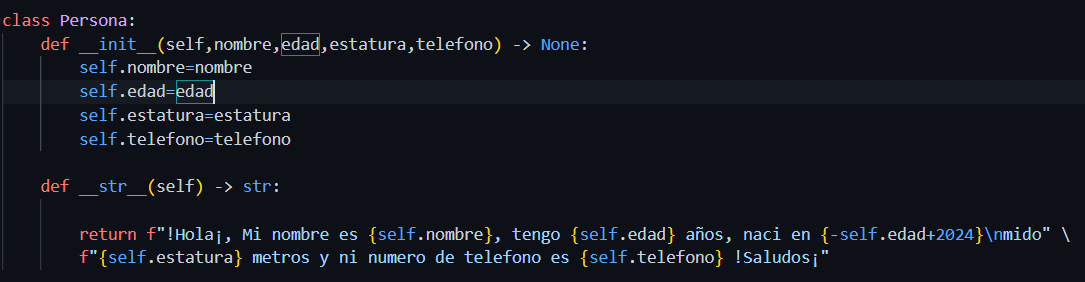
\includegraphics[width = .8\textwidth]{01.png}
 			\captionof{figure}{\label{fig:IPN}Creacion de la clase persona con sus respectivos atributos} 
 			
		\end{center} 
\end{figure}
	
En la figura 1 se puede observar la creacion de la clase persona con sus respectivos atributos  y su metodo llamado str el cual nos devolvera el texto similar al que es requerido en el problema
	


En este problema se requiere que el ususario es el que ingrese los datos de las 3 personas. Esto supone un reto para el programa, debido a que los datos que ingrese deben estar dentro de los rangos de una persona normal, para evitar que ingrese datos incorrectos o diferentes a los solicitados se generaron 4 funciones con el fin de verificar que el usuaio al menos ingrese datos en campos validos, a continuacion presentamos las 4 funciones generadas

\begin{enumerate}
\item{Funcion pedir nombre}
Esta funcions se encarga de recibir un nombre como argumento y analizar si dicho nombre contiene todos sus caracteres de tipo alfabetico, con ayuda de la funcion .isalpha(), la cual se encarga de analizar la cadena y devolver True o False en cada caso, esto esta dentro de un ciclo while, el cual se encarga de ejecutarse hasta que el usuario ingrese un nombre aceptable para el programa

\begin{figure}[H]
		\begin{center}
 			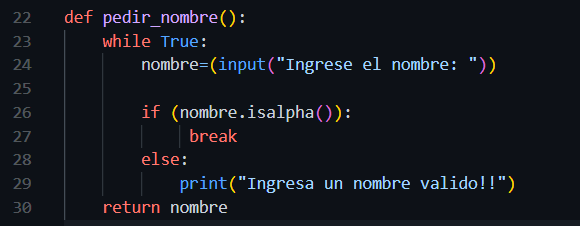
\includegraphics[width = .8\textwidth]{02.png}
 			\captionof{figure}{\label{fig:IPN}Funcion para ingresar un nombre valido} 
 			
		\end{center} 
\end{figure}

\item{Funcion pedir edad}
Para esta funcion vamos a considerar un rango de edad que este entre los 0 y 100 años,  en caso de que el usuario ingrese una edad que no este en ese rango el programa volvera a pedir al usuario que ingrese la edad
\begin{figure}[H]
		\begin{center}
 			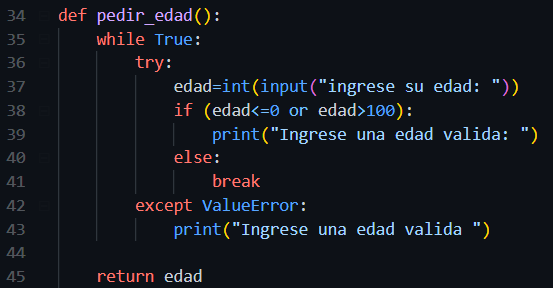
\includegraphics[width = .8\textwidth]{03.png}
 			\captionof{figure}{\label{fig:IPN}Funcion para ingresar una edad valido} 
 			
		\end{center} 
\end{figure}


\item{Funcion pedir estatura} Para esta funcion lo que hacemos es etablecer un limite que este entre 0 y 2.15 metros, alguno otro valor fuera de este rango volvera a preguntar la estatura

\begin{figure}[H]
		\begin{center}
 			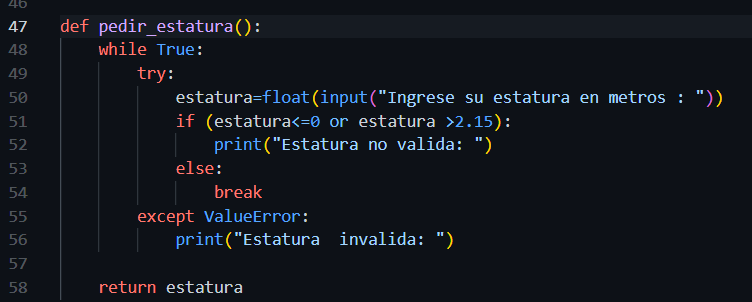
\includegraphics[width = .8\textwidth]{04.png}
 			\captionof{figure}{\label{fig:IPN}Funcion para una estatura aceptable} 
 			
		\end{center} 
\end{figure}

\item{Funcion pedir telefono}
Para esta funcion vamos a considerar un numero valido al menos en mexico con 10 digitos, con el uso de la funcion len, la cual  le pasamos como argumento una cadena donde esta guardado el numero ingresado por el usuario, esta funcion analiza el numero de caracteres, en el caso donde se ingrese un numero con diferentes caracteristicas la sentencia se va a seguir ejecutando hasta el ingreso de uno valido


\begin{python}[caption=Funcion para pedir un numero de telefono ,label=python_example]
def pedir_telefono():
    while True:
        try:
            numero=int(input("Ingrese su numero de telefono (10 digitos): \n"))
            if (numero<0 or (len(str(numero))<10)):
                print("Ingres un numero valido")
            else :
                break
        except ValueError:
            print("Ingrese un numero valido: ")
    return numero

\end{python}



\end{enumerate}

Ahora que hemos terminado de hacer las funciones que nos ayudaran a 
pedir los datos requeridos vamos con la parte de carga de codigo e impresion de valores: \\
Primero iniciamos con la creacion de una tupla llamada personas, despues iteramos en un ciclo for de 1 hasta 3, donde conforme avanza i, en pantalla se mostrara el numero de persona en la que esteremos ingresando los datos, recalquemos que la variable persona es un objeto de tipo Persona, y aqui es donde añadimos las funciones que definimos anteriormente, las funciones iran en los argumentos del objeto persona. posteriormente la variable persona es añadida a la tupla.\\
Por ulstimo usamos un ciclo for para mostrar en pantalla las presentaciones de cada persona en consola

\begin{python}[caption=Carga de valores e impresion de resultados,label=python_example]
personas=[]

for i in range(3):
    print(f"--------PERSONA {i+1}")
    persona=Persona(pedir_nombre(),pedir_edad(),pedir_estatura(), pedir_telefono())
    personas.append(persona)
    os.system("cls")

os.system("cls")   
for i in range(3):
    print(personas[i])


\end{python}

\subsection{Programa 2.}
Ahora analisemos el programa numero 2, el cual consiste en solicitar al usuario El nombre y datos del profesor, asi como de n alumnos, para posteriormente imprimirlos en una tipo lista. La practica sugiere usar 3 clases las cuales son Alumno, Profesor, Lista, para esta practica yo lo desrrolle de otra forma ya que se me hizo mas factible desarrollarlo con las siguientes clases

\begin{python}[caption=Clases utilizadas en esta practica,label=python_example]
class Persona:
    def __init__(self,nombre,ap,am,fecha_n) -> None:
        self.nombre=nombre
        self.ap=ap
        self.am=am
        self.fecha_n=fecha_n

class Alumno(Persona):
    def __init__(self, nombre,ap,am,fecha_n,boleta,grupo,carrera,correo) -> None:
        super().__init__(nombre,ap,am,fecha_n)

        self.boleta=boleta
        self.grupo=grupo
        self.carrera=carrera
        self.correo=correo

    def __str__(self) -> str:
        return f"{self.ap} {self.am},{self.nombre}--{self.boleta}--{self.fecha_n}\n"\
        f"{self.carrera}--{self.grupo}--{self.correo}"

class Profesor(Persona):
    def __init__(self,nombre,no_empleado) -> None:
        super().__init__(nombre,ap=None,am=None,fecha_n=None)
        self.no_empleado=no_empleado

    def __str__(self) -> str:
        return f"\n\nProfesor:  {self.nombre}\nNo. Empleado: {self.no_empleado}"

\end{python}
En la listeng 3, observamos las clases usadas en este programa se basan en una clase principal la cual es Persona, esta clase tiene los atributos de nombre,apellidos, y fecha de nacimiento las cuales son heredadas a las clases hijas de Alumno y Profesor, ambas clases agregan sus propios atributos, como profesor agrega su numero de empleado, y alumnos agrega los datos de carrera y algunos de contacto, tambien agregan el metodo str, con la finalidad de devolver una cadena tipo string que muestre todos los atributos proporcionados por el usuario\\

Ademas agregamos funcciones similares a las del problema 1, solo las mencionaremos y daremos una breve explicacion de cada funcion para no alargar mucho el texto con elementos muy similares
\begin{figure}[H]
		\begin{center}
 			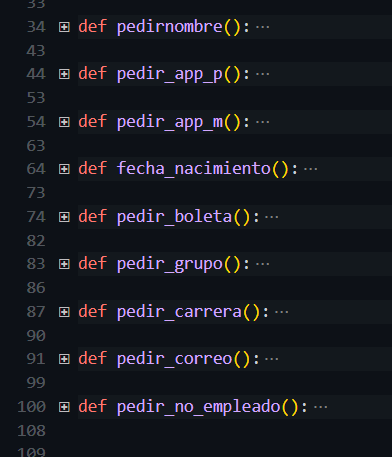
\includegraphics[width = .4\textwidth]{11.png}
 			\captionof{figure}{\label{fig:IPN}Funciones usadas en el programa 2} 
 			
		\end{center} 
\end{figure}

\begin{enumerate}
\item Pedir nombre es similar al anterior, ahora puede admitir 2 nombres y de igual forma analizarlos para comprobar que tenga caracteres validos
\item pedir apellido paterno: analiza la entrada y pide un apellido valido, de igual forma para el apellido materno
\item fecha de nacimiento: con ayuda de la libreria datatime, podemos verificar si la entrada de la fecha es valida o invalida y volverla a solicitar
\item Boleta: admite solo caracteres enteros
\item grupo: para esta funcion puede ser una mezcla de caracteres alfanumericos, buscando una respueste a grupos similares en UPIITA
\item Carrera: Permite el ingreso de tipo string
\item correo: para validar esta entrada nos respaldamos en el caracter @ para darla como valida
\item Numero de empleado: unicamente admite entrada de tipo numerico
\end{enumerate}

Para llevar a cabo el alamcenamiento de datos, vamos a necesittar una tupla, y como el ejemplo anterior con un ciclo while vamos a salir del bucle cuando ingresemos n, podemos observarlo en la siguiente figura
\begin{figure}[H]
		\begin{center}
 			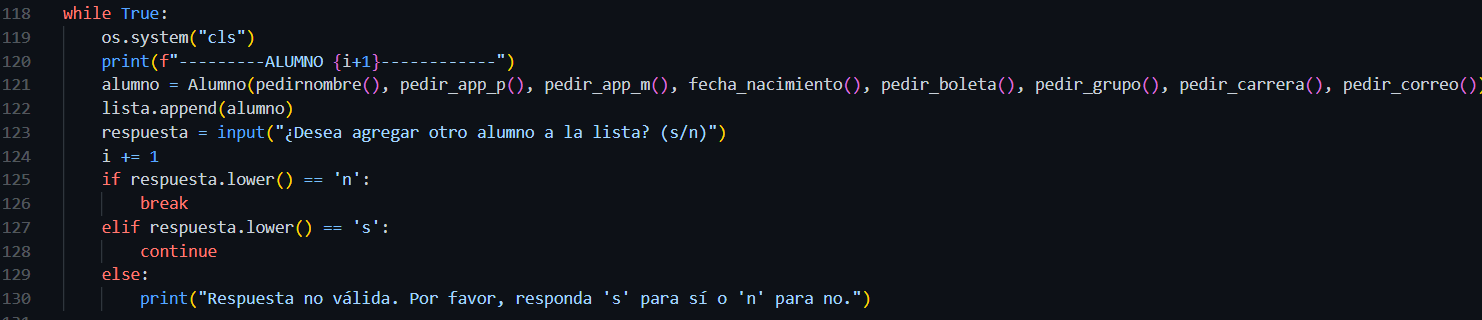
\includegraphics[width = .9\textwidth]{12.png}
 			\captionof{figure}{\label{fig:IPN}Ciclo para guardar los objetos en una tupla} 
 			
		\end{center} 
\end{figure}
Finalmente se imprimen la lista con un ciclo for y con ayuda del metodo str que se asigna en cada clase (alumno y profesor)
\begin{python}[caption=Imprime la lista en consola ,label=python_example]
for i in range(len(lista)):
    print(lista[i])
    print("-"*50)

print(f"Total de alumnos inscritos: {len(lista)}")


\end{python}

\section{Ejecucion.}
\subsection{Problema 1.}
Ahora vamos a ejecutar el primer programa y veamos que nos imprime en pantalla: 
\begin{figure}[H]
		\begin{center}
 			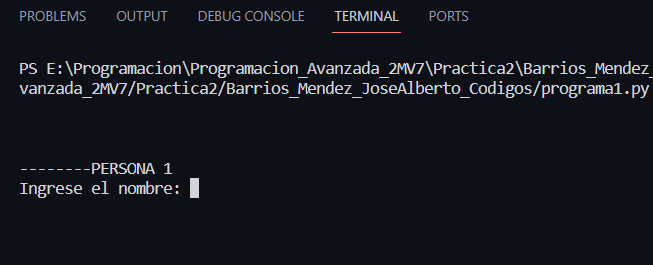
\includegraphics[width = .8\textwidth]{07.png}
 			\captionof{figure}{\label{fig:IPN}Ejecucion del programa 1} 
 			
		\end{center} 
\end{figure}

vamos a intentar ingresar algunos nombres con otros caracteres para ver como responde el programa ante estas entradas

\begin{figure}[H]
		\begin{center}
 			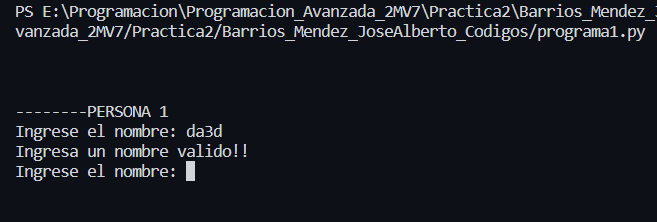
\includegraphics[width = .8\textwidth]{08.png}
 			\captionof{figure}{\label{fig:IPN}Ejecucion del programa 1} 
 			
		\end{center} 
\end{figure}

En la figura 7, podemos observar que al ingresar un nombre valido, nos pregunta la edad, de la misma forma testeamos algunos valores que no estan dentro del rango anteriormente definidios, de igual forma realizamos lo mismo para la altura y para el numero de telefono, al ingresar al final el numero de telefono correcto nos arrojara a la segunda persona, y despues a la tercera, llenando los datos de forma aleatoria observemos el resultado: 


\begin{figure}[H]
		\begin{center}
 			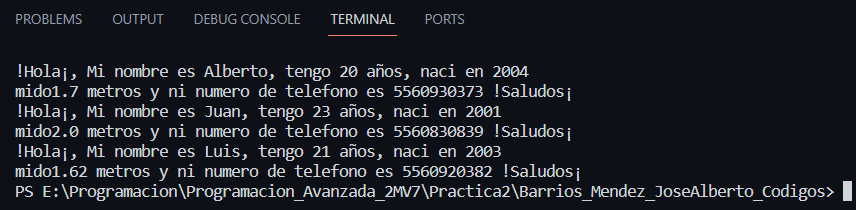
\includegraphics[width = .8\textwidth]{10.png}
 			\captionof{figure}{\label{fig:IPN}Resultado final del programa 1} 
 			
		\end{center} 
\end{figure}
\subsection{Programa 2}
Veamos el resultado al ejecutar el programa

\begin{figure}[H]
		\begin{center}
 			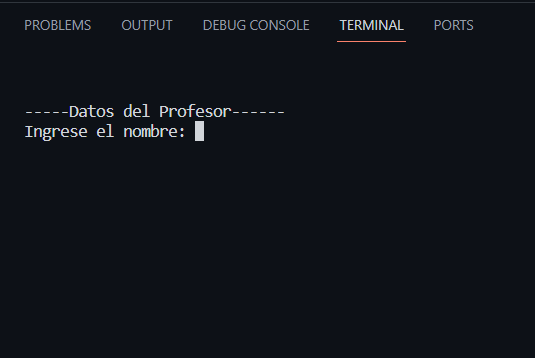
\includegraphics[width = .4\textwidth]{13.png}
 			\captionof{figure}{\label{fig:IPN}Ejecucion del programa 2} 
 			
		\end{center} 
\end{figure}

Veamos que nos aparece la instruccion para ingresar el nombre del profesor, posteriormente tambien pedira  el numero de empleado
\begin{figure}[H]
		\begin{center}
 			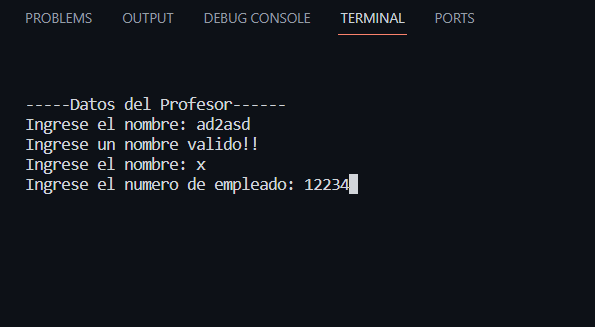
\includegraphics[width = .6\textwidth]{14.png}
 			\captionof{figure}{\label{fig:IPN}Ingreso de datos de1 profesor } 
 			
		\end{center} 
\end{figure}

Una vez que ingresemos los datos del profesor nos mandara a ingresar los datos de los alumnos, a continuacion presentamos un caso, ademas de testear las respuestas para provar el codigo:
\begin{figure}[H]
		\begin{center}
 			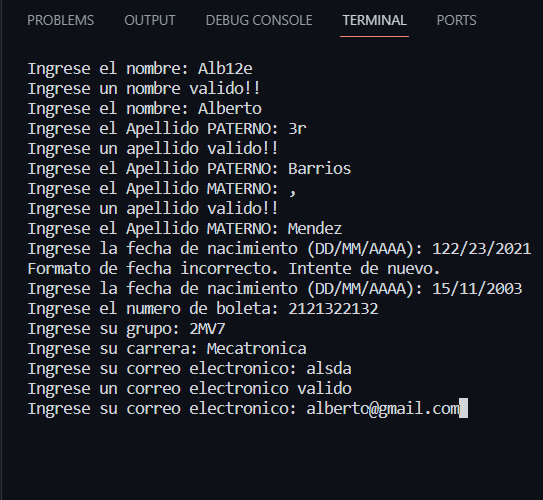
\includegraphics[width = .6\textwidth]{15.png}
 			\captionof{figure}{\label{fig:IPN} Ingreso de datos de un estudiante, variando las respuestas} 
 			
		\end{center} 
\end{figure}

Para mostrar el resultado final, consideramos 2 alumnos ingresados par poder verificar que el programa funciona correctamente.
\begin{figure}[H]
		\begin{center}
 			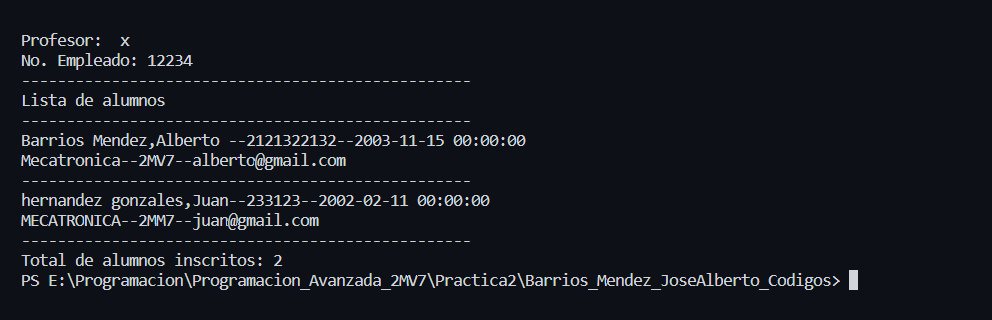
\includegraphics[width = .6\textwidth]{16.png}
 			\captionof{figure}{\label{fig:IPN} resultado final del programa 2}
 			 
 			
		\end{center} 
\end{figure}


\section{Conclusiones.}

Al concluir esta practica donde tratamos algunos temas sobre Programacion orientada a objetos me doy cuenta que es muy eficiente este tipo de programacion ya que nos permite crear bastantes objetos a partir de varias clases con ayuda de la herencia, ademas de su facil manejo del lenguaje lo que lo convierte en una herramienta muy util para nuestro perfil como futoros ingenieros mecatronicos

%%%%%%% Bibliografía %%%%%%%%    

%\appendix  
%\clearpage % o \cleardoublepage
%\addappheadtotoc 
%\appendixpage

%\section{Anexos 1.}




%\section{Anexos 2.}


 

\end{document}
